% Options for packages loaded elsewhere
\PassOptionsToPackage{unicode}{hyperref}
\PassOptionsToPackage{hyphens}{url}
%
\documentclass[
]{article}
\usepackage{amsmath,amssymb}
\usepackage{lmodern}
\usepackage{iftex}
\ifPDFTeX
  \usepackage[T1]{fontenc}
  \usepackage[utf8]{inputenc}
  \usepackage{textcomp} % provide euro and other symbols
\else % if luatex or xetex
  \usepackage{unicode-math}
  \defaultfontfeatures{Scale=MatchLowercase}
  \defaultfontfeatures[\rmfamily]{Ligatures=TeX,Scale=1}
\fi
% Use upquote if available, for straight quotes in verbatim environments
\IfFileExists{upquote.sty}{\usepackage{upquote}}{}
\IfFileExists{microtype.sty}{% use microtype if available
  \usepackage[]{microtype}
  \UseMicrotypeSet[protrusion]{basicmath} % disable protrusion for tt fonts
}{}
\makeatletter
\@ifundefined{KOMAClassName}{% if non-KOMA class
  \IfFileExists{parskip.sty}{%
    \usepackage{parskip}
  }{% else
    \setlength{\parindent}{0pt}
    \setlength{\parskip}{6pt plus 2pt minus 1pt}}
}{% if KOMA class
  \KOMAoptions{parskip=half}}
\makeatother
\usepackage{xcolor}
\IfFileExists{xurl.sty}{\usepackage{xurl}}{} % add URL line breaks if available
\IfFileExists{bookmark.sty}{\usepackage{bookmark}}{\usepackage{hyperref}}
\hypersetup{
  pdftitle={MovieLens Project},
  pdfauthor={Berkalp Altay},
  hidelinks,
  pdfcreator={LaTeX via pandoc}}
\urlstyle{same} % disable monospaced font for URLs
\usepackage[margin=1in]{geometry}
\usepackage{graphicx}
\makeatletter
\def\maxwidth{\ifdim\Gin@nat@width>\linewidth\linewidth\else\Gin@nat@width\fi}
\def\maxheight{\ifdim\Gin@nat@height>\textheight\textheight\else\Gin@nat@height\fi}
\makeatother
% Scale images if necessary, so that they will not overflow the page
% margins by default, and it is still possible to overwrite the defaults
% using explicit options in \includegraphics[width, height, ...]{}
\setkeys{Gin}{width=\maxwidth,height=\maxheight,keepaspectratio}
% Set default figure placement to htbp
\makeatletter
\def\fps@figure{htbp}
\makeatother
\setlength{\emergencystretch}{3em} % prevent overfull lines
\providecommand{\tightlist}{%
  \setlength{\itemsep}{0pt}\setlength{\parskip}{0pt}}
\setcounter{secnumdepth}{-\maxdimen} % remove section numbering
\usepackage{booktabs}
\usepackage{longtable}
\usepackage{array}
\usepackage{multirow}
\usepackage{wrapfig}
\usepackage{float}
\usepackage{colortbl}
\usepackage{pdflscape}
\usepackage{tabu}
\usepackage{threeparttable}
\usepackage{threeparttablex}
\usepackage[normalem]{ulem}
\usepackage{makecell}
\usepackage{xcolor}
\ifLuaTeX
  \usepackage{selnolig}  % disable illegal ligatures
\fi

\title{MovieLens Project}
\author{Berkalp Altay}
\date{January 12, 2022}

\begin{document}
\maketitle

{
\setcounter{tocdepth}{3}
\tableofcontents
}
\newpage

\hypertarget{introduction}{%
\subsection{1. Introduction}\label{introduction}}

This project aims to build a recommendation system using the MovieLens
10M dataset.

\hypertarget{dataset}{%
\subsubsection{1.1. Dataset}\label{dataset}}

In this MovieLens dataset, there are about 10 Million movie ratings with
6 different categories associated with each rating.

These 6 categories are the following:

\begin{itemize}
\item
  Title of the movie
\item
  Movie ID
\item
  Genre of the movie
\item
  User ID
\item
  Rating (from 0.5 to 5 in increments of 0.5 with 5 being the best
  rating possible)
\item
  Timestamp for the date and time of the rating
\end{itemize}

There are approximately 70000 unique users and 10000 unique movies.\\
The genres include Comedy, Adventure, Drama, and so on.\\
Also, the release date of a movie is included in parentheses at the end
of a title.

\hypertarget{evaluation-criteria}{%
\subsubsection{1.2. Evaluation Criteria}\label{evaluation-criteria}}

In the next sections, the data will be explored and recommendation
systems will be built using the data. The recommendation system will be
evaluated using the Root Mean Squared Error (RMSE).\\

The RMSE formula is as follows:

\[\mbox{RMSE} = \sqrt{\frac{1}{n}\sum_{t=1}^{n}\hat{y}_i^2-y_i^2}\]\\
In this formula, \(\hat{y}_i\) represents the predicted ratings based on
the recommendation system while \(y_i\) represents the actual ratings
from the dataset.\\
The lower the RMSE, the better the model is. For this project, an RMSE
lower than 0.86490 is the ultimate target. This ultimate RMSE evaluation
will be based on a validation set that will be used only for model
evaluation at the end in Section \texttt{3.\ Results}.\\
Using the validation set, the Regularized Movie \& User \& Release Year
\& Timestamp Model, the final model in this project, reaches an RMSE of
\textbf{0.8648589}. This meets the ultimate target.

\hypertarget{analysis}{%
\subsection{2. Analysis}\label{analysis}}

\hypertarget{data-exploration}{%
\subsubsection{2.1. Data Exploration}\label{data-exploration}}

The 10 million movie ratings are initially divided into two datasets:
\emph{edx} and \emph{validation} with the \emph{edx} dataset containing
approximately 90\% of the data while the \emph{validation} dataset
contains the remaining 10\%.\\
The rows of both the \emph{edx} and \emph{validation} datasets are
entries for different ratings.\\
Also, both the \emph{edx} and \emph{validation} datasets have 6
columns.\\

\begin{table}[H]

\caption{\label{tab:Table 1: Columns names with explanation}Columns}
\centering
\fontsize{11}{13}\selectfont
\begin{tabular}[t]{|>{}c|||>{}l|}
\hline
columns & column\_explanations\\
\hline
userId & Unique identifier for each user\\
\hline
movieId & Unique identifier for each movie\\
\hline
title & Title of a movie\\
\hline
genres & Genre of a movie - multiple genres are concatenated with a | sign such as Comedy|Romance\\
\hline
rating & Rating given by a specific user to a specific movie\\
\hline
timestamp & Date and time associated with each rating\\
\hline
\end{tabular}
\end{table}

The \emph{validation} set will be used in Section \texttt{3.\ Results}
as a final hold-out test set for only reporting the RMSE of the final
model. Therefore, a training set and a test set seem necessary while
building and testing models.~ To that end, the \emph{edx} set has been
divided into \emph{edxTrain} and \emph{edxTest} sets. The \emph{edxTest}
set has been created as the same size as that of the \emph{validation}
set. So, both the \emph{edxTest} and \emph{validation} sets have
approximately 1 million movie ratings (i.e.~both have 10\% of the
original MovieLens 10M dataset) while the \emph{edxTrain} set has
approximately 8 million movie ratings.

\hypertarget{data-preparation-and-data-visualization}{%
\subsubsection{2.2. Data Preparation and Data
Visualization}\label{data-preparation-and-data-visualization}}

\hypertarget{data-preparation-phase}{%
\paragraph{2.2.1. Data Preparation Phase}\label{data-preparation-phase}}

\hfill\break
\hfill\break
After the data exploration phase, we see that the title column contains
the release year for each movie. For example, the title for Pulp Fiction
is listed as \texttt{Pulp\ Fiction\ (1994)}.\\
Also, the timestamp is not in a human-readable format.\\
First, the release year for each movie will be extracted from the title
column and added to \emph{edxTrain} and \emph{edxTest} sets as a
column.\\
Second, the timestamp column will be converted to a human-readable form
and the year will be extracted. This will provide the year in which the
rating was given.

Third, the RMSE formula for the evaluation purposes will be defined as
per the definition given in Section \texttt{1.2.\ Evaluation\ Criteria}.

After these changes, we can see some rows of the \emph{edxTrain} and
\emph{edxTest} sets below.

\begin{table}[H]

\caption{\label{tab:Table 2: first 3 rows of edxTrain set}First 3 rows of edxTrain set}
\centering
\fontsize{6.7}{8.7}\selectfont
\begin{tabular}[t]{|>{}c|||>{}c|||>{}c|||>{}c|||>{}c|||>{}c|||>{}c|||>{}c|}
\hline
userId & movieId & rating & timestamp & title & genres & release\_year & rating\_year\\
\hline
\cellcolor{gray!6}{1} & \cellcolor{gray!6}{185} & \cellcolor{gray!6}{5} & \cellcolor{gray!6}{838983525} & \cellcolor{gray!6}{Net, The (1995)} & \cellcolor{gray!6}{Action|Crime|Thriller} & \cellcolor{gray!6}{1995} & \cellcolor{gray!6}{1996}\\
\hline
1 & 329 & 5 & 838983392 & Star Trek: Generations (1994) & Action|Adventure|Drama|Sci-Fi & 1994 & 1996\\
\hline
\cellcolor{gray!6}{1} & \cellcolor{gray!6}{355} & \cellcolor{gray!6}{5} & \cellcolor{gray!6}{838984474} & \cellcolor{gray!6}{Flintstones, The (1994)} & \cellcolor{gray!6}{Children|Comedy|Fantasy} & \cellcolor{gray!6}{1994} & \cellcolor{gray!6}{1996}\\
\hline
\end{tabular}
\end{table}

\begin{table}[H]

\caption{\label{tab:Table 3: first 3 rows of edxTest set}First 3 rows of edxTest set}
\centering
\fontsize{8}{10}\selectfont
\begin{tabular}[t]{|>{}c|||>{}c|||>{}c|||>{}c|||>{}c|||>{}c|||>{}c|||>{}c|}
\hline
userId & movieId & rating & timestamp & title & genres & release\_year & rating\_year\\
\hline
\cellcolor{gray!6}{1} & \cellcolor{gray!6}{122} & \cellcolor{gray!6}{5} & \cellcolor{gray!6}{838985046} & \cellcolor{gray!6}{Boomerang (1992)} & \cellcolor{gray!6}{Comedy|Romance} & \cellcolor{gray!6}{1992} & \cellcolor{gray!6}{1996}\\
\hline
1 & 292 & 5 & 838983421 & Outbreak (1995) & Action|Drama|Sci-Fi|Thriller & 1995 & 1996\\
\hline
\cellcolor{gray!6}{1} & \cellcolor{gray!6}{316} & \cellcolor{gray!6}{5} & \cellcolor{gray!6}{838983392} & \cellcolor{gray!6}{Stargate (1994)} & \cellcolor{gray!6}{Action|Adventure|Sci-Fi} & \cellcolor{gray!6}{1994} & \cellcolor{gray!6}{1996}\\
\hline
\end{tabular}
\end{table}

\hypertarget{data-visualization}{%
\paragraph{2.2.2. Data Visualization}\label{data-visualization}}

\hypertarget{average-rating}{%
\subparagraph{2.2.2.1. Average Rating}\label{average-rating}}

\hfill\break
First, we notice that every movie has a different average rating. Below,
we can see this looking at Figure 1 created using the \emph{edx} set.

\begin{center}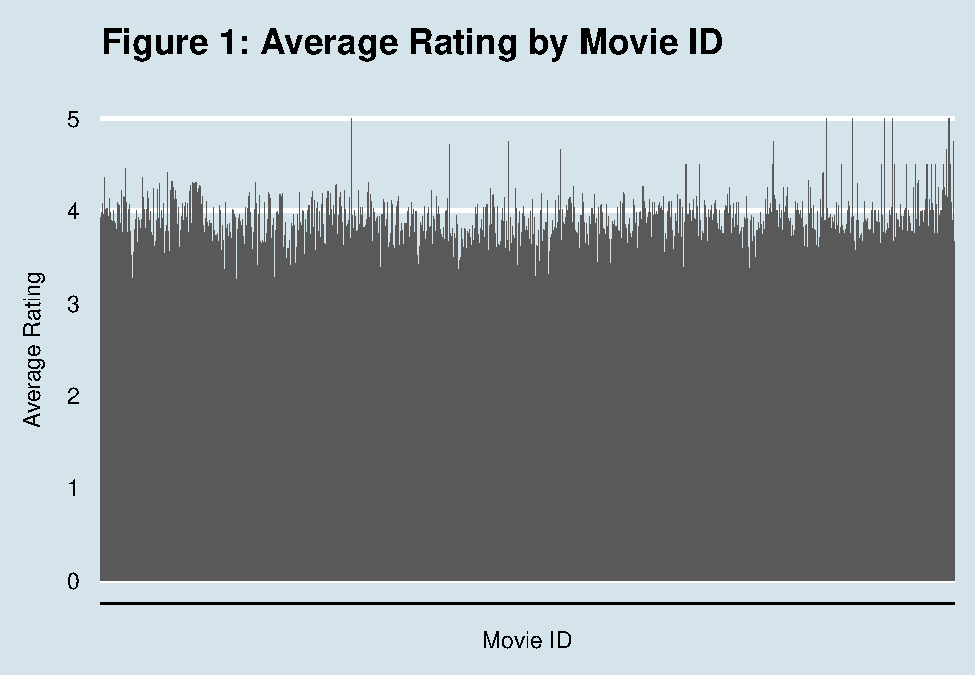
\includegraphics[width=0.75\linewidth,height=0.5\textheight]{MovieLens_Project_files/figure-latex/Figure 1 - Average Rating by Movie ID-1} \end{center}

Second, we notice that every user has a different average rating. Below,
we can see this looking at Figure 2 created using the \emph{edx} set.

\begin{center}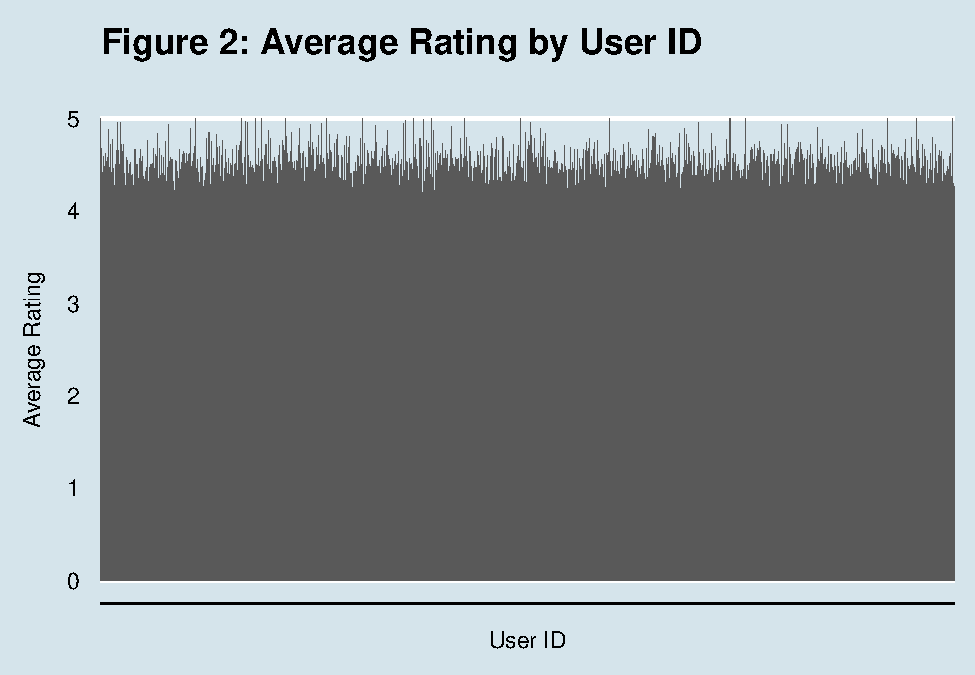
\includegraphics[width=0.75\linewidth,height=0.5\textheight]{MovieLens_Project_files/figure-latex/Figure 2 - Average Rating by User ID-1} \end{center}

Third, we notice that the movies released between around 1930 and 1985
seem to have higher ratings than the ones released after 1985. Below, we
can see this looking at Figure 3 created using the \emph{edx} set.

\begin{center}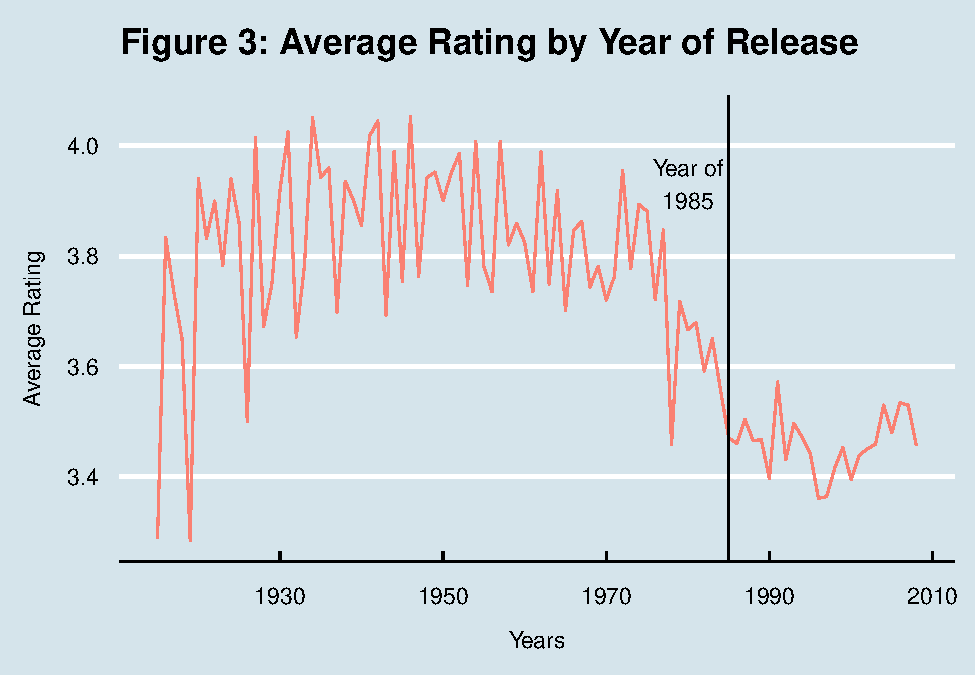
\includegraphics[width=0.75\linewidth,height=0.5\textheight]{MovieLens_Project_files/figure-latex/Figure 3 - Average Rating by Year of Release-1} \end{center}

Fourth, we notice that the movies rated before 2000 seem to have higher
ratings than the ones released after 2000. Below, we can see this
looking at Figure 4 created using the \emph{edx} set.

\begin{center}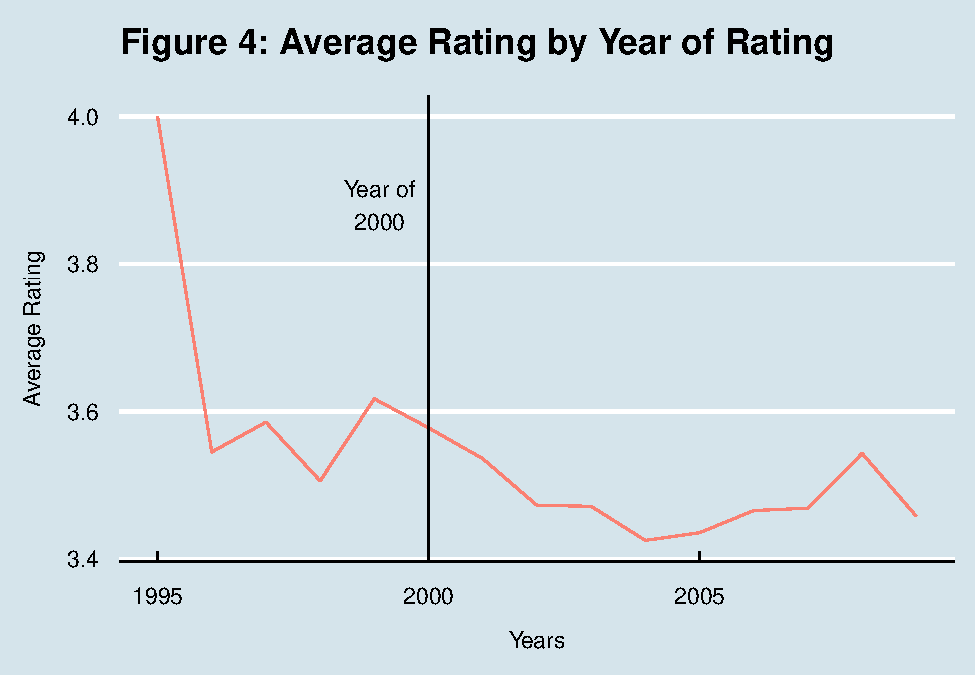
\includegraphics[width=0.75\linewidth,height=0.5\textheight]{MovieLens_Project_files/figure-latex/Figure 4 - Average Rating by Year of Rating-1} \end{center}

As seen in the Figures above, there is significant variability in
ratings by movie ID, user ID, year of release, and year of rating.

\hypertarget{frequency}{%
\subparagraph{2.2.2.2. Frequency}\label{frequency}}

\hfill\break
\hfill\break
First, not all movies are rated as frequently as others. In Tables 4 and
5 below, you can see top 5 and bottom 5 movies in the \emph{edx} set by
the frequency of ratings, respectively. For example, in the \emph{edx}
set, \texttt{Pulp\ Fiction} was rated 31362 times while
\texttt{100\ Feet} was rated only once.

\begin{table}[H]

\caption{\label{tab:Table 4: Top 5 Movies by Rating Frequency}Top 5 Movies by Rating Frequency}
\centering
\fontsize{11}{13}\selectfont
\begin{tabular}[t]{|>{}c|||>{}c|}
\hline
title & count\\
\hline
\cellcolor{gray!6}{Pulp Fiction (1994)} & \cellcolor{gray!6}{31362}\\
\hline
Forrest Gump (1994) & 31079\\
\hline
\cellcolor{gray!6}{Silence of the Lambs, The (1991)} & \cellcolor{gray!6}{30382}\\
\hline
Jurassic Park (1993) & 29360\\
\hline
\cellcolor{gray!6}{Shawshank Redemption, The (1994)} & \cellcolor{gray!6}{28015}\\
\hline
\end{tabular}
\end{table}

\begin{table}[H]

\caption{\label{tab:Table 5: Bottom 5 Movies by Rating Frequency}Bottom 5 Movies by Rating Frequency}
\centering
\fontsize{11}{13}\selectfont
\begin{tabular}[t]{|>{}c|||>{}c|}
\hline
title & count\\
\hline
\cellcolor{gray!6}{1, 2, 3, Sun (Un, deuz, trois, soleil) (1993)} & \cellcolor{gray!6}{1}\\
\hline
100 Feet (2008) & 1\\
\hline
\cellcolor{gray!6}{4 (2005)} & \cellcolor{gray!6}{1}\\
\hline
Accused (Anklaget) (2005) & 1\\
\hline
\cellcolor{gray!6}{Ace of Hearts (2008)} & \cellcolor{gray!6}{1}\\
\hline
\end{tabular}
\end{table}

Second, not all users rate as frequently as others. In Tables 6 and 7
below, you can see top 5 and bottom 5 user IDs in the \emph{edx} set by
the number of times they have rated, respectively. For example, in the
\emph{edx} set, the user with an ID number of 59269 rated 6616 times
while the user with an ID number of 62516 rated only 10 times.

\begin{table}[H]

\caption{\label{tab:Table 6: Top 5 Users by Rating Frequency}Top 5 Users by Rating Frequency}
\centering
\fontsize{11}{13}\selectfont
\begin{tabular}[t]{|>{}c|||>{}c|}
\hline
userId & count\\
\hline
\cellcolor{gray!6}{59269} & \cellcolor{gray!6}{6616}\\
\hline
67385 & 6360\\
\hline
\cellcolor{gray!6}{14463} & \cellcolor{gray!6}{4648}\\
\hline
68259 & 4036\\
\hline
\cellcolor{gray!6}{27468} & \cellcolor{gray!6}{4023}\\
\hline
\end{tabular}
\end{table}

\begin{table}[H]

\caption{\label{tab:Table 7: Bottom 5 Users by Rating Frequency}Bottom 5 Users by Rating Frequency}
\centering
\fontsize{11}{13}\selectfont
\begin{tabular}[t]{|>{}c|||>{}c|}
\hline
userId & count\\
\hline
\cellcolor{gray!6}{62516} & \cellcolor{gray!6}{10}\\
\hline
22170 & 12\\
\hline
\cellcolor{gray!6}{15719} & \cellcolor{gray!6}{13}\\
\hline
50608 & 13\\
\hline
\cellcolor{gray!6}{901} & \cellcolor{gray!6}{14}\\
\hline
\end{tabular}
\end{table}

\hypertarget{modeling-approach}{%
\subsubsection{2.3. Modeling Approach}\label{modeling-approach}}

In this section, various models will be built. In all these models,
\emph{edxTest} set will be used with the RMSE function for evaluation of
the model since the evaluation of the final model using the
\emph{validation} set will be conducted in the \texttt{3.\ Results}
Section.

\hypertarget{baseline-mean-model}{%
\paragraph{2.3.1. Baseline Mean Model}\label{baseline-mean-model}}

\hfill\break
\hfill\break
In this model, we assume that every movie has the same rating and that
same rating is the average (i.e.~mean) rating of all movies.\\
\strut \\
The formula for the Baseline Mean Model:\\
\[Y = \mu+ \epsilon\]\\
where \(\mu\) stands for the average rating for all movies and
\(\epsilon\) stands for independent errors sampled from the same
distribution centered at zero.

Therefore, this model assigns a rating of about \textbf{3.512417} to
every movie.

The RMSE for the Baseline Mean model using the \emph{edxTest} set is
around \textbf{1.059487}. We can interpret this result as missing the
actual rating stars by around 1.06 stars. This is far from perfect and
also misses the ultimate target of \textbf{0.86490}.

\hypertarget{movie-model}{%
\paragraph{2.3.2. Movie Model}\label{movie-model}}

\hfill\break
\hfill\break
In this model, we start taking movies into account. In particular, we
know and use the fact that not all movies are rated the same, as seen in
Figure 1 in Section \texttt{2.2.}. Therefore, we account for the
variability of ratings due to movies themselves.\\
\strut \\
The formula for the Movie Model:\\
\[Y_{m} = \mu+b_{m}+ \epsilon\]\\
where \(\mu\) stands for the average rating for all movies and \(b_m\)
stands for the average rating for movie \(m\), also called the movie
effect while \(\epsilon\) stands for independent errors sampled from the
same distribution centered at zero.

The RMSE for the Movie Model using the \emph{edxTest} set is around
\textbf{0.9434865}. While this is a substantial improvement from the
RMSE of \textbf{1.059487} for the Baseline Mean Model, it misses the
ultimate target of \textbf{0.86490} and can be further improved.

\hypertarget{movie-user-model}{%
\paragraph{2.3.3. Movie \& User Model}\label{movie-user-model}}

\hfill\break
\hfill\break
In this model, we take both movies and users into account when it comes
to predicting ratings. In particular, we know and use the fact that not
all users give the same ratings.\\
\strut \\
The formula for the Movie \& User Model:\\
\[Y_{m, u} = \mu+b_{m}+b_{u}+ \epsilon\]\\
where \(\mu\) stands for the average rating for all movies, \(b_m\)
stands for the average rating for movie m, also called the movie effect,
\(b_u\) stands for the user effect while \(\epsilon\) stands for
independent errors sampled from the same distribution centered at zero.

The RMSE for the Movie \& User Model using the \emph{edxTest} set is
around \textbf{0.8655475}. While this is a great improvement from the
RMSE of \textbf{1.059487} for the Baseline Mean Model and the RMSE of
\textbf{0.9434865} for the Movie Model, it misses the ultimate target of
\textbf{0.86490} and can be further improved.

\hypertarget{movie-user-year-model}{%
\paragraph{2.3.4. Movie \& User \& Year
Model}\label{movie-user-year-model}}

\hfill\break
\hfill\break
While the ratings are greatly influenced by users and movies, there
seems to be some variation in ratings by the year of release. In Figure
3 in Section \texttt{2.2.}, we can see that people gave higher ratings
to movies released between around 1930 and 1985 than the ones released
from 1985 onward.\\
\strut \\
The formula for the Movie \& User \& Year Model:~
\[Y_{m, u, y} = \mu+b_{m}+b_{u}+b_{y}+ \epsilon\]\\
where \(\mu\) stands for the average rating for all movies, \(b_m\)
stands for the average rating for movie m, also called the movie effect,
\(b_u\) stands for the user effect, \(b_y\) stands for the effect of the
year of release while \(\epsilon\) stands for independent errors sampled
from the same distribution centered at zero.

The RMSE for the Movie \& User \& Year Model using the \emph{edxTest}
set is around \textbf{0.8651656}. Although this comes closer to the
ultimate target of \textbf{0.86490} than the RMSE of \textbf{0.8655475}
for the Movie \& User Model, it can still be improved.

\hypertarget{movie-user-year-timestamp-model}{%
\paragraph{2.3.5. Movie \& User \& Year \& Timestamp
Model}\label{movie-user-year-timestamp-model}}

\hfill\break
While the ratings are greatly influenced by users and movies, there
seems to be some variation in ratings by the year of rating (i.e.~year
of Timestamp). In Figure 4 in Section \texttt{2.2.}, we can see some
variation in ratings by the year of rating by a user.\\
\strut \\
The formula for the Movie \& User \& Year \& Timestamp Model:\\
\[Y_{m, u, y, t} = \mu+b_{m}+b_{u}+b_{y}+b_{t}+ \epsilon\]\\
where \(\mu\) stands for the average rating for all movies, \(b_m\)
stands for the average rating for movie m, also called the movie effect,
\(b_u\) stands for the user effect, \(b_y\) stands for the effect of the
year of release, \(b_t\) stands for the effect of the year of rating
(i.e.~timestamp effect) while \(\epsilon\) stands for independent errors
sampled from the same distribution centered at zero.

The RMSE for the Movie \& User \& Year \& Timestamp Model using the
\emph{edxTest} set is around \textbf{0.8650907}. Although this comes
closer to the ultimate target of \textbf{0.86490} than the RMSE of
\textbf{0.8651656} for the Movie \& User \& Year Model, it can still be
improved.

\hypertarget{regularized-movie-user-release-year-timestamp-model}{%
\paragraph{\texorpdfstring{2.3.6. Regularized Movie \& User \& Release
Year \& Timestamp Model\\
}{2.3.6. Regularized Movie \& User \& Release Year \& Timestamp Model }}\label{regularized-movie-user-release-year-timestamp-model}}

While the last model is a good improvement, we can improve the results
further.~In Tables 4 and 5, we see that some movies are rated more
frequently than others. Likewise, some users rate more frequently than
others while some years of release and years of rating have more movie
ratings than others. In this case, a smaller frequency of rating can
introduce bias into the model. For example, a movie might be rated 5.0
but have only one rating. In this case, our prediction of a 5.0 rating
introduces a bias into our model.\\
To that end, we can modify the RMSE to penalize large estimates coming
from small samples.\\
\strut \\
The formula for the RMSE with regularization:

\[\frac{1}{N} \sum_{m, u, y, t} (y_{m, u, y, t} - \mu - b_m - b_u - b_y - b_t)^2 + \lambda(\sum_{m}b_m^2 + \sum_{u}b_u^2 + \sum_{y}b_y^2 + \sum_{t}b_t^2)\]\\
The term on the left hand side of the plus sign is the mean squared
error and the term on the right hand side is a penalty term for larger
\(b\)'s. So, we have to pick b's to minimize this equation.\\
\strut \\
Multiple values of lambda can be tried to find the best solution. To
tune lambda this way, only the \emph{edxTest} set will be used since the
\emph{validation} set is reserved only for the final evaluation of the
model.

While more lambda values offer greater tuning for the regularization,
more lambda values result in more computationally expensive processes.
Therefore, the sequence of numbers from 0 to 20 in increments of 1 is
chosen as the lambda values to strike a balance between better tuning
and computational expense.\\
The RMSE values obtained for these lambda values are given in Figure 5
below.

\begin{center}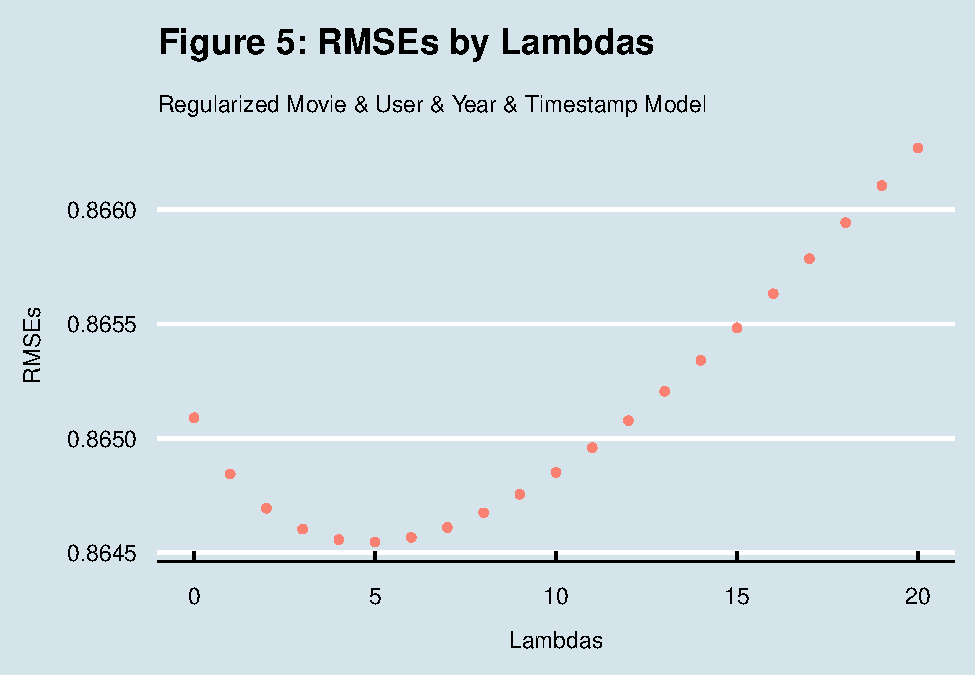
\includegraphics[width=0.75\linewidth,height=0.5\textheight]{MovieLens_Project_files/figure-latex/Plot - RMSEs by Lambdas-1} \end{center}

As seen in the \texttt{RMSEs\ by\ Lambdas} graph above, the smallest
RMSEs occurs when lambda is equal to 5. Using 5 as the lambda and the
\emph{edxTest} set, the RMSE for the Regularized Movie \& User \& Year
\& Timestamp Model is around \textbf{0.8645478} beating the ultimate
target of \textbf{0.86490}.

\hypertarget{results}{%
\subsection{3. Results}\label{results}}

Now, the \emph{validation} set can be used to evaluate the Regularized
Movie \& User \& Year \& Timestamp Model, the final model. The best
lambda that results in the minimum RMSE for the model was obtained using
the model on the \emph{edxTest} set in Section \texttt{2.3.6.} and will
be used for the evaluation purpose of the \emph{validation} set.

The Regularized Movie \& User \& Year \& Timestamp Model has a RMSE of
\textbf{0.8648589} which beats the ultimate target of
\textbf{0.86490}.\\
For reference, the RMSE of all models using the \emph{validation} set
can be found below:

\begin{table}[H]

\caption{\label{tab:Table 8: Validation Results Table for All models}RMSEs of All Models Using Validation Set}
\centering
\fontsize{13}{15}\selectfont
\begin{tabular}[t]{|>{}c|||>{}c|}
\hline
Model & RMSE\\
\hline
\cellcolor{gray!6}{Baseline Mean Model} & \cellcolor{gray!6}{1.0612018}\\
\hline
Movie Model & 0.9439998\\
\hline
\cellcolor{gray!6}{Movie \& User Model} & \cellcolor{gray!6}{0.8659094}\\
\hline
Movie \& User \& Year Model & 0.8655625\\
\hline
\cellcolor{gray!6}{Movie \& User \& Year \& Timestamp Model} & \cellcolor{gray!6}{0.8654879}\\
\hline
Regularized Movie \& User \& Year \& Timestamp Model & 0.8648589\\
\hline
\end{tabular}
\end{table}

As seen in Table 8 above, the ultimate model was built by incorporating
new features in every step of the model building process.\\

The model performance ultimately improved from an RMSE of
\textbf{1.0612018} (i.e.~Baseline Mean Model) to the final RMSE of
\textbf{0.8648589}.

\hypertarget{conclusion}{%
\subsection{4. Conclusion}\label{conclusion}}

In this project, the MovieLens 10M dataset was sucessfully used to build
a recommendation system model.\\

This report introduced the MovieLens dataset, explored its properties,
introduced newly developed features from existing ones and visualized
the data.\\

Then, a model was built bit by bit from the rudimentary approach of
assigning the overall movie average to all movies to a regularized model
that incorporated movies, users, years of release for the movies and the
years of ratings by users that decreased the error between a predicted
rating and an actual rating.\\

The model improved the most when the model incorporated movieId and
userId. Adding the year of release (i.e.~Year component of the models)
and the year of rating (i.e.~Timestamp component of the models) led to a
slight improvement. Regularization also helped in this regard as it
penalized big estimates of effects from small sample sizes.\\

All in all, the final model achieved the goal of reaching an RMSE below
\textbf{0.86490}.

Some limitations of this project is that it did not employ methods such
as matrix factorization or artificial neural networks. Such methods can
be used to discern relationships among data that are not readily
recognizable. Therefore, any future work can further improve on this
report by employing such methods.

\end{document}
